\lab{Poisson's equation}{Poisson's equation}
\label{lab:poisson2d}
 
Suppose that we want to describe the distribution of heat throughout a region $\Omega$.
Let $g(x)$ represent the temperature on the boundary of $\Omega$ ($\partial \Omega$), and let $h(x)$ represent the initial heat distribution at time $t = 0$.
If we let $f(x,t)$ represent any heat sources/sinks in $\Omega$, then the flow of heat can be described by the boundary value problem (BVP)
\begin{align}
	\begin{split}
		& { } u_t = \triangle u + f(x,t), \quad x \in \Omega, \quad t >0,\\
		& { }u(x,t) = h(x), \quad x \in \partial \Omega, \\
		& { }u(x,0) = g(x).
	\end{split}
\end{align}
When the source term $f$ does not depend on time, there is often a steady-state heat distribution $u_{\infty}$ that is approached as $t \to \infty$.
This steady state $u_{\infty}$ is a solution of the BVP
\begin{align}
	\begin{split}
		& { }  \triangle u + f(x) = 0, \quad x \in \Omega,\\
		& { }u(x,t) = h(x), \quad x \in \partial \Omega.
	\end{split}
\end{align}

This last partial differential equation, $\triangle u = -f$, is called Poisson's equation.
This equation is satisfied by the steady-state solutions of many other evolutionary processes.
Poisson's equation is often used in electrostatics, image processing, surface reconstruction, computational fluid dynamics, and other areas. 


\section*{Poisson's equation in two dimensions}
 Consider Poisson's equation together with Dirichlet boundary conditions on a rectangular  domain $R = [a,b] \times [c,d]$:
 \begin{align}
	\begin{split}
 	u_{xx} + u_{yy} &= f,\quad x \text{ in } R \subset \mathbb{R}^2,\\
 	u &= g, \quad x \text{ on } \partial R.
	\end{split}\label{eqn:2d_poisson}
\end{align}
Let $a = x_{-1}, x_0, \ldots, x_{N-1} = b$ be a partition of $[a,b]$, and let $c = y_{-1}, y_0, \ldots, y_{N-1} = d$ be a partition of $[c,d]$.
Suppose that there are $N+1$ evenly spaced points, so that $N$ is the number of subintervals in each dimension, and $x_i, y_j$ are given by 
\begin{align*}
	x_i &= a + (i+1)h, \\
	y_j &= c + (j+1)k,
\end{align*}
% for $i,j = 0, \ldots, N-2$, 
where $h = x_i-x_{i-1},$ $k = y_i-y_{i-1}$.
We look for an approximation $U_{i,\,j}$ on the grid $\{(x_{i},y_{j})\}_{i,j=-1}^{N-1}$.

Recalling that 
 \begin{align*}
 \triangle u(x_i,y_j) &= u_{xx}(x_i,y_j) + u_{yy}(x_i,y_j) \\
&= \frac{u(x_{i+1},y_{j}) - 2u(x_{i},y_{j})+ u(x_{i-1},y_{j})}{h^2} \\
 & \qquad{}+ 
 \frac{u(x_{i},y_{j+1}) - 2u(x_{i},y_{j})+ u(x_{i},y_{j-1})}{k^2} + \mathcal{O}(h^2 + k^2).
 \end{align*}
we replace $\triangle $ with the finite difference operator $\triangle_{h,k}$:
 \begin{align*}
 \triangle_{h,k} U_{ij} &:= \frac{U_{i+1,\,j} - 2U_{i,\,j} + U_{i-1,\,j}}{h^2} + \frac{U_{i,\,j+1} - 2U_{i,\,j}+ U_{i,\,j-1}}{k^2}.
% &= \frac{1}{h^2}(U_{i-1,\,j} + U_{i+1,\,j} + U_{i,\,j-1} + U_{i,\,j+1}-4U_{i,\,j}).
 \end{align*}
By applying this operator at the interior points of our grid, we obtain the equations  
\[
\triangle_{h,k} U_{ij} = f_{ij}, \quad i,j = 0,\ldots,N-2.
\]

By ordering these equations first in $i$, and secondly in $j$, we can write them in matrix form as
\[AU + p +  q  = f,\]
where the vector $U$ above is given by 
\[U = \begin{bmatrix} U^0 \\ U^1 \\ \\ U^{N-2} \end{bmatrix} \text{ where } U^j = 
\begin{bmatrix} U_{0,\,j} \\ U_{1,\,j} \\ \\ U_{N-2,\,j} \end{bmatrix} \text{ for each } j,\quad 0\leq j \leq N-2.\]
The entries of $f$ are ordered similarly.
The matrix $A$ is block tridiagonal, given by 
\[\frac{1}{h^2}
\begin{bmatrix}
T & I & &  &\\
I &T & I & &\\
&\ddots  & \ddots & \ddots & \\
&  & I & T & I \\
&  &  & I & T\end{bmatrix},\]
where $I$ is the $N-1\times N-1$ % $m\times m$
identity matrix and $T$ is the tridiagonal matrix
\[\begin{bmatrix}
-4 & 1 & &  &\\
1 &-4 & 1 & &\\
&\ddots  & \ddots & \ddots & \\
&  & 1 & -4 & 1 \\
&  &  & 1 & -4 \end{bmatrix}.\]


% \[U = \begin{bmatrix} U^1 \\ U^2 \\ \\ U^m \end{bmatrix} \text{ where } U^j = 
% \begin{bmatrix} U_{1,\,j} \\ U_{2,\,j} \\ \\ U_{m,\,j} \end{bmatrix} \text{ for each } j, 1\leq j \leq m\]
% So $U^j$ represents the $j$th row of interior points in our grid, where $y_j = jh$
$p$ and $q$ come from the boundary conditions of \eqref{eqn:2d_poisson}, and are given by 
\[p = \begin{bmatrix} p^0 \\ \ldots \\ \\ p^{N-2} \end{bmatrix}, \quad  q = \begin{bmatrix} q^0 \\ \ldots \\ \\ q^{N-2} \end{bmatrix},\]
where 
\[p^j = \frac{1}{h^2} \begin{bmatrix} g_{-1,\,j} \\ 0 \\ \vdots \\0\\ g_{N-1,\,j} \end{bmatrix} ,\quad 0 \leq j \leq N-2,\]
and 
\[q^0 = \frac{1}{h^2}\begin{bmatrix} g_{0,-1}  \\ g_{1,-1} \\ \vdots \\ g_{N-3,-1}\\ g_{N-2,-1} \end{bmatrix}, \quad q^{N-2} = \frac{1}{h^2}\begin{bmatrix} g_{0,N-1} \\ g_{1,N-1} \\ \vdots \\ g_{N-3,N-1}\\ g_{N-2,N-1} \end{bmatrix}, \quad q^{j} = \begin{bmatrix} 0 \\ 0 \\ \vdots \\ 0 \\ 0 \end{bmatrix} ,\quad 1 \leq j \leq N-3.\]

% The vector $q$ is given by $u = [q^0 \ldots q^{N-2}]^T$, %   $u = [q^1 \ldots q^m]^T$,
% where 
% \[q^j = \frac{1}{h^2} \begin{bmatrix} g_{0,\,j} \\ 0 \\ \vdots \\0\\ g_{m+1,\,j} \end{bmatrix} , \,\,\, 2 \leq j \leq m-1\]
% and 
% \[q^1 = \frac{1}{h^2}\begin{bmatrix} g_{1,0} + g_{0,1} \\ g_{2,0} \\ \vdots \\ g_{m-1,0}\\ g_{m,0} + g_{m+1,1}\end{bmatrix}, \quad q^m = \frac{1}{h^2}\begin{bmatrix} g_{1,m+1} + g_{0,m}\\ g_{2,m+1} \\ \vdots \\ g_{m-1,m+1}\\ g_{m,m+1} + g_{m+1,m}\end{bmatrix}\]

% \begin{problem}
% Find the solution $u$ of the 2D Laplace equation $\Delta u = 0$ on the unit 
% square $[0,1]\times [0,1] \subset \mathbb{R}^2,$ subject to the (Dirichlet) condition that 
% $u(x,y) = x^3$ on the boundary. 
% 	 
% Graph your solution, and demonstrate convergence of the numerical approximation by 
% creating a log-log plotof the error $E(h).$
% \end{problem}

% \begin{problem}
% Find the solution $u$ of the 2D Poisson equation with the given Dirichlet boundary conditions:
% \begin{align*}
% 	\Delta u &= -\pi^2 \sin(\pi x)\sin(\pi y), \quad (x,y) \in [0,1]\times [0,1], \\
% 	u(x,0) &= 1-x, \\
% 	u(x,1) &= 1-2x, \\
% 	u(0,y) &= 1, \\
% 	u(1,y) &= -y. 
% \end{align*}
% 
% Graph your solution, and demonstrate convergence of the numerical approximation by 
% creating a log-log plot of the error $E(h).$
% \end{problem}

% The matrix $A$ is sparse, and so we can use several functions from the package \texttt{scipy.sparse.linalg}.
% In particular, we use the functions \texttt{spdiags} and \texttt{spsolve}.
%  
%  \begin{verbatim}
% D1,D2,D3 = -4*np.ones((1,m**2)), np.ones((1,m**2)), np.ones((1,m**2)) 
% Dm1, Dm2 = np.ones((1,m**2)), np.ones((1,m**2))
% for j in range(0,D2.shape[1]):
% 	if (j%m)==m-1: 
% 		D2[0,j]=0
% 	if (j%m)==0: 
% 		D3[0,j]=0
% diags = np.array([0,-1,1,-m,m])
% data = np.concatenate((D1,D2,D3,Dm1,Dm2),axis=0) # This stacks up rows
% A = 1./h**2.*spdiags(data, diags, m**2,m**2).asformat('csr') # This ap
%  \end{verbatim}
 
\begin{comment}
\subsection{2D Heat Equation}
Recall that the collection of finite difference equations
\[\nabla^2_h U_{ij} = 0, \quad 1 \leq i,j\leq m\]
can be written in matrix form as
\[AU + q  = 0\]

The Crank-Nicolson method for the 2D heat equation is given by 
\[U_{i,\,j}^{n+1}- U_{i,\,j}^{n} = \frac{\Delta t}{2}(\nabla_h^2 U_{i,\,j}^{n} + \nabla_h^2 U_{i,\,j}^{n+1}) \text{ for each } 1 \leq i,j \leq m\]
is a second order accurate in both space and time. Basically we're using a midpoint scheme in time, 
and a trapezoidal scheme in space. The resulting method is implicit, and can be written in matrix form as 
\begin{align*}
	IU^{n+1} &= IU^n + \frac{\Delta t}{2}(AU^n + q + AU^{n+1} + q)\\
	(I - \frac{\Delta t}{2}A)U^{n+1}&= (I + \frac{\Delta t}{2}A)U^n + \Delta t q
\end{align*}

% TODO: What size must the time step be to ensure stability? 

We will need to take many time steps, where many equations must be solved with the matrix $(I - \frac{\Delta t}{2}A)$.
The function \texttt{factorized} from \texttt{scipy.sparse.linalg} computes the LU decomposition of the matrix.
This decomposition reduces the time required for solving consecutive time steps.
\end{comment}

\section*{Poisson's Equation and Conservative Forces}
Poisson's equation is used in physics to describe the scalar potential of a conservative force.
In general
\[ \Delta V = - f\]
where $V$ is the scalar potential of the force (the potential energy a particle would have at that point), and $f$ is a source term.
Examples of conservative forces include Newton's law of gravity (where matter become the source term) and Coulomb's Law, which gives the force between two charge particles (where charge is the source term).

In electrostatics in the absence of magnetic fields it can be shown from Maxwell's equations that the scalar potential $V$ of the electric force (or electric potential field) satisfies
\[  \Delta V = -\frac{\rho}{\epsilon_0},\]
where $\rho$ is the charge density and $\epsilon_0$ is the permissivity of free space,
which is a constant that we'll leave as $1$. 

A nonzero $V$ at a point will typically cause a charged particle to move to a lower potential,
thereby changing $\rho$ and the solution to $V$.
However, in the following analysis we'll assume the charges (or charge distribution) is fixed, for a naive approximation.

One simple application of the electric potential is to calculate basic properties of simple molecules, using a charge distibution to calculate the electric potential field.
We'll assume that the electrons produce clouds of charge centered around the atoms, roughly appoximated by a Boltzmann Distribution $\rho = q e^{-r}$, where $q$ is the relative charge of the atom and $r$ is the distance from the atom. 
To make this easier, we'll make a function (\li{rho1}) to calculate the $\rho$ value at a certain point in space based on the position of an atom and it's relative charge. 
We'll make another function (\li{rhoSum}) to give the total charge density as the superposition of a list of atoms (ignoring the complex interations between the atoms).

\begin{lstlisting}
#definitions for atoms position and charges
#the angle the hydrogen atoms make
theta = 106.0/180.0*np.pi
#Length of the two branches
A = 1.0
# Hydrogen 1 (x0,y0,q)
# Hydrogen 2 
# Oxygen
water = ((-np.sin(theta / 2) * A, 0, 1),
         (np.sin(theta / 2) * A, 0, 1),
         (0, -np.cos(theta / 2) * A, -2))

def rho1(x, y, atom):
    return atom[2] * np.exp(-np.sqrt((x - atom[0])**2 + (y - atom[1])**2))

def rhoSum(x,y,atoms):
    return np.sum([rho1(x,y,atom) for atom in atoms],axis=0)

# Generate a color dictionary for use with LinearSegmentedColormap.
# It places red and blue at the min and max values of data
# and white when data is zero.
def genDict(data):
    zero = 1 / (1 - np.max(data) / np.min(data))
    cdict = {'red':[(0.0,  1.0, 1.0),
                   	(zero,  1.0, 1.0),
                   	(1.0,  0.0, 0.0)],
         'green':  [(0.0,  0.0, 0.0),
                   	(zero,  1.0, 1.0),
                   	(1.0,  0.0, 0.0)],
         'blue':   [(0.0,  0.0, 0.0),
                   	(zero,  1.0, 1.0),
                   	(1.0,  1.0, 1.0)]}
    return cdict
X = np.linspace(-5, 5, 100)
X, Y = np.meshgrid(X, X)
# Generate the grid of rho values.
Rho = rhoSum(X, Y, water)
plt.imshow(Rho, cmap =  mcolors.LinearSegmentedColormap('cmap', genDict(Rho)))
plt.colorbar()
plt.show()
\end{lstlisting}
The function \li{genDict} scales the color values to be white when the charge density is zero.
This is mostly to help visualize where there are neutrally charged zones by forcing them to be white.
You may find it useful to also apply it when you solve for the electric  potential.

\begin{figure}
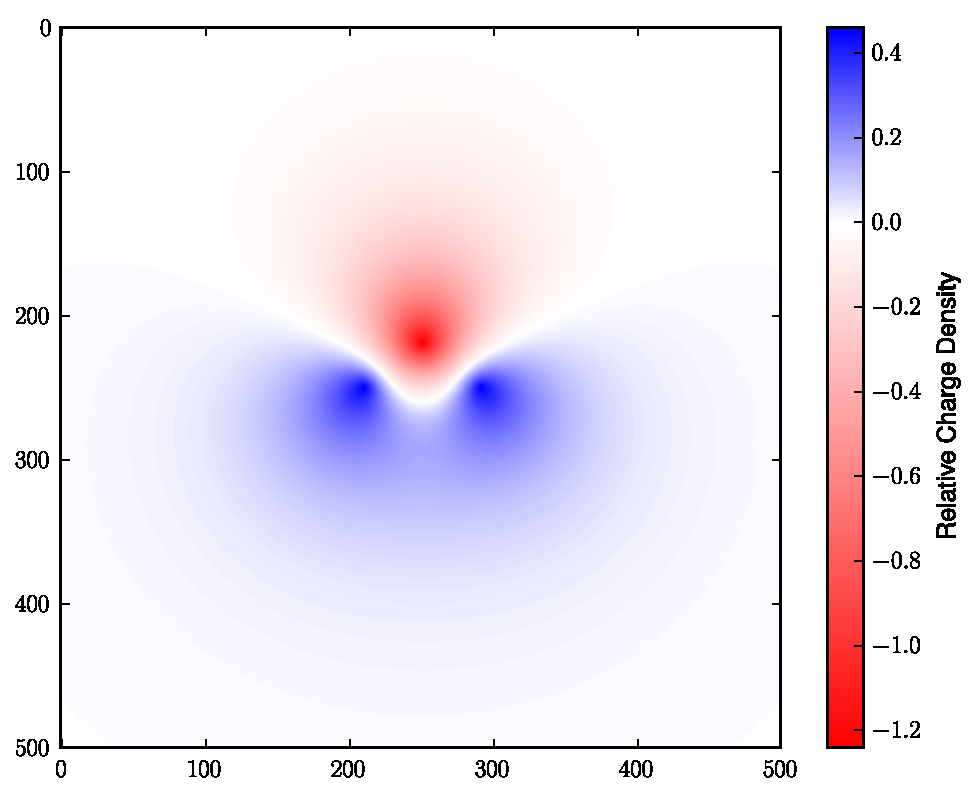
\includegraphics[width=\textwidth]{waterRho.pdf}
\caption{Relative charge density of an H$_2$O molecule}
\end{figure}

With a function for $\rho$, we can solve Poisson's equation for the electric potential field.
\begin{problem}
Solve for the electric potential $V$
\[\Delta V = -\rho(x,y)\]
The electric potential is usually defined to go to zero at inifinity.
We can approximate this using $V=0$ at the boundry conditions on $[-5,5]\times [-5,5]$.
Solve and plot the electric potential of water, using the definition for the atoms above.

\textit{Due to the size of $A$, this is best done using sparse matrices}
\end{problem}

\begin{problem}
Solve for the electric potential of a CO$_2$ molecule.

CO$_2$ can be modeled as two atoms of relative charge $-1$ placed at $x=-1$ and $x=1$ on the $x$ axis and a third atom with relative charge $2$ at the origin.
Simply reuse your code from the last problem with new definitions for the atoms using the template for a water molecule.

If the molecules are moving slowly (ie. when the temperature is low) electrostatic forces will dominate molecular interactions.
Molecules will want to align themselves in the lowest energy configuration, or the lowest electric potential.
Positive potentials will overlap themselves with negative potentials.
From the electric potential plots you obtain, how do you think the molecules will arrange themselves when the temperature is cold, when they form an ice?
\end{problem}

\begin{figure}
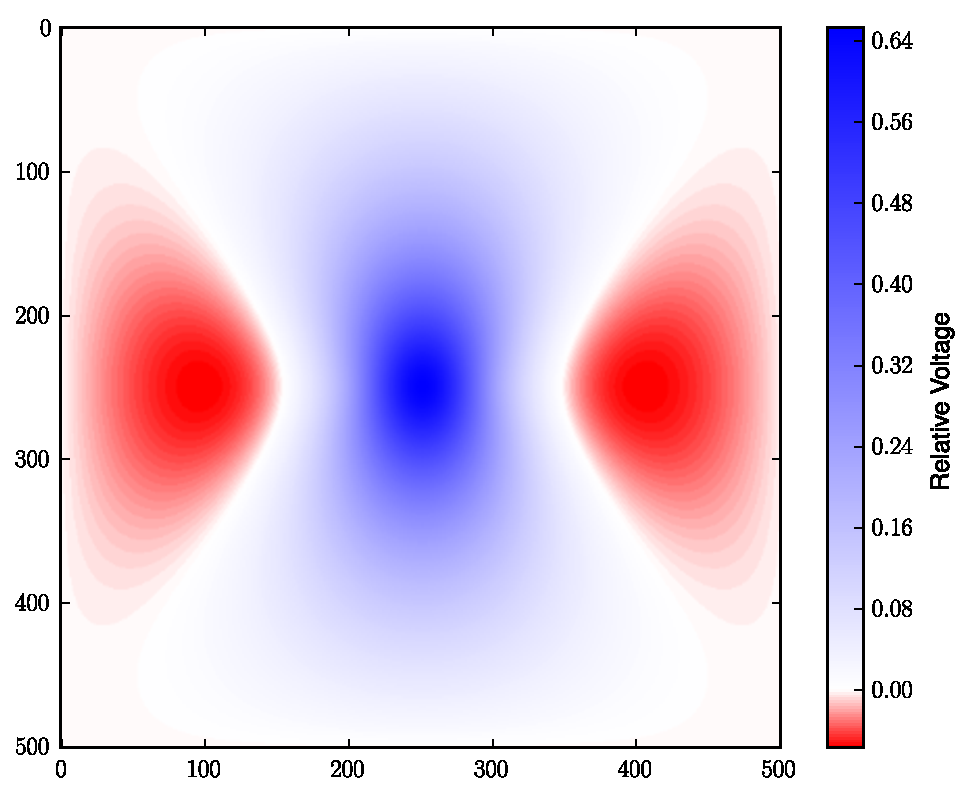
\includegraphics[width=\textwidth]{co2V.pdf}
\caption{Relative electric potential field of a CO$_2$ molecule}
\end{figure}